\chapter{}

\section*{Из воспоминаний C. Л. Корчиковой (Клейн), И. Д. Бабенко, Н. Б. Канторович}

До войны, в 30-е годы в доме № 2/6 по Хоромному тупику существовал Красный уголок для жильцов дома и их детей. Он был организован усилиями энергичного человека~-- управдома Ивана Максимовича Калиша и находился в подвальном помещении подъезда №5. Большую работу по организации кружков вела Евдокия Ивановна Варзар. В Красном уголке постоянно работала библиотека (книги выдавала и беседовала о книгах Елена Николаевна Лоренц), демонстрировались фильмы, тогда черно-белые и немые (регулярно приезжала кинопередвижка), и работали кружки: драмкружок с приглашенным режиссером,   танцевальный   кружок, детский   оркестр; гордостью    Красного уголка стал    кружок автомобилестроения,   в   котором дети под руководством специалиста конструировали     педальные   автомобили   из   фанеры и деталей, которые поставлял ГИРД (Государственный   институт ракетных двигателей), находившийся в   районе   Красных   ворот;   в этот институт для детей   была проведена  экскурсия,    которая  произвела на  них    большое   впечатление. На этих автомобилях несколько мальчиков и   девочек совершили   въезд  на Красную площадь    в   праздник МЮДа   (Международный   юношеский день 1 сентября).

Красный уголок был местом постоянного общения  детей, где они могли обменяться впечатлениями о прочитанных книгах,    прослушанных   по   радио интересных передачах (телевизоров тогда не было), поиграть на пианино или на бильярде, подготовиться      к очередному концерту: концерты,   на   которые всегда приходили   родители и   другие жильцы дома, готовились    к каждому празднику, ставились спектакли, к которым дети сами шили костюмы и делали декорации,   играл   детский оркестр,   дети     пели, танцевали и читали стихи. К каждому празднику все   дети получали поздравительные открытки и подарки:   небольшой   мешочек   с кондитерскими изделиями.

Красный уголок стал любимым местом общения детей и их культурного времяпрепровождения и развития.


Кроме того, Красный уголок был также местом собраний жильцов дома, общественности, где обсуждались разные насущные проблемы. Просмотр фильмов обычно предназначался совместно для детей и взрослых.

\indent

В настоящее время, когда дети нередко предоставлены самим себе и не имеют должного общения, представляется очень актуальным возродить заведение типа прежнего Красного уголка и создать условия для его функционирования, предоставив для этого подходящее помещение, а конкретно-свободное подвальное помещение в подъезде № 5 дома № 2/6 по Хоромному тупику.


\begin{figure}[ht!]
    \begin{minipage}{100mm}
        \includegraphics[width=100mm]{inc/85/1}
        \footnotesize{\textit{Соня Клейн, Люба Абрамович, Нина Клейн. Конец 40-х.}}
     \end{minipage}
\end{figure}

\vspace{10pt}

\begin{figure}[h!]
\begin{minipage}{100mm}
    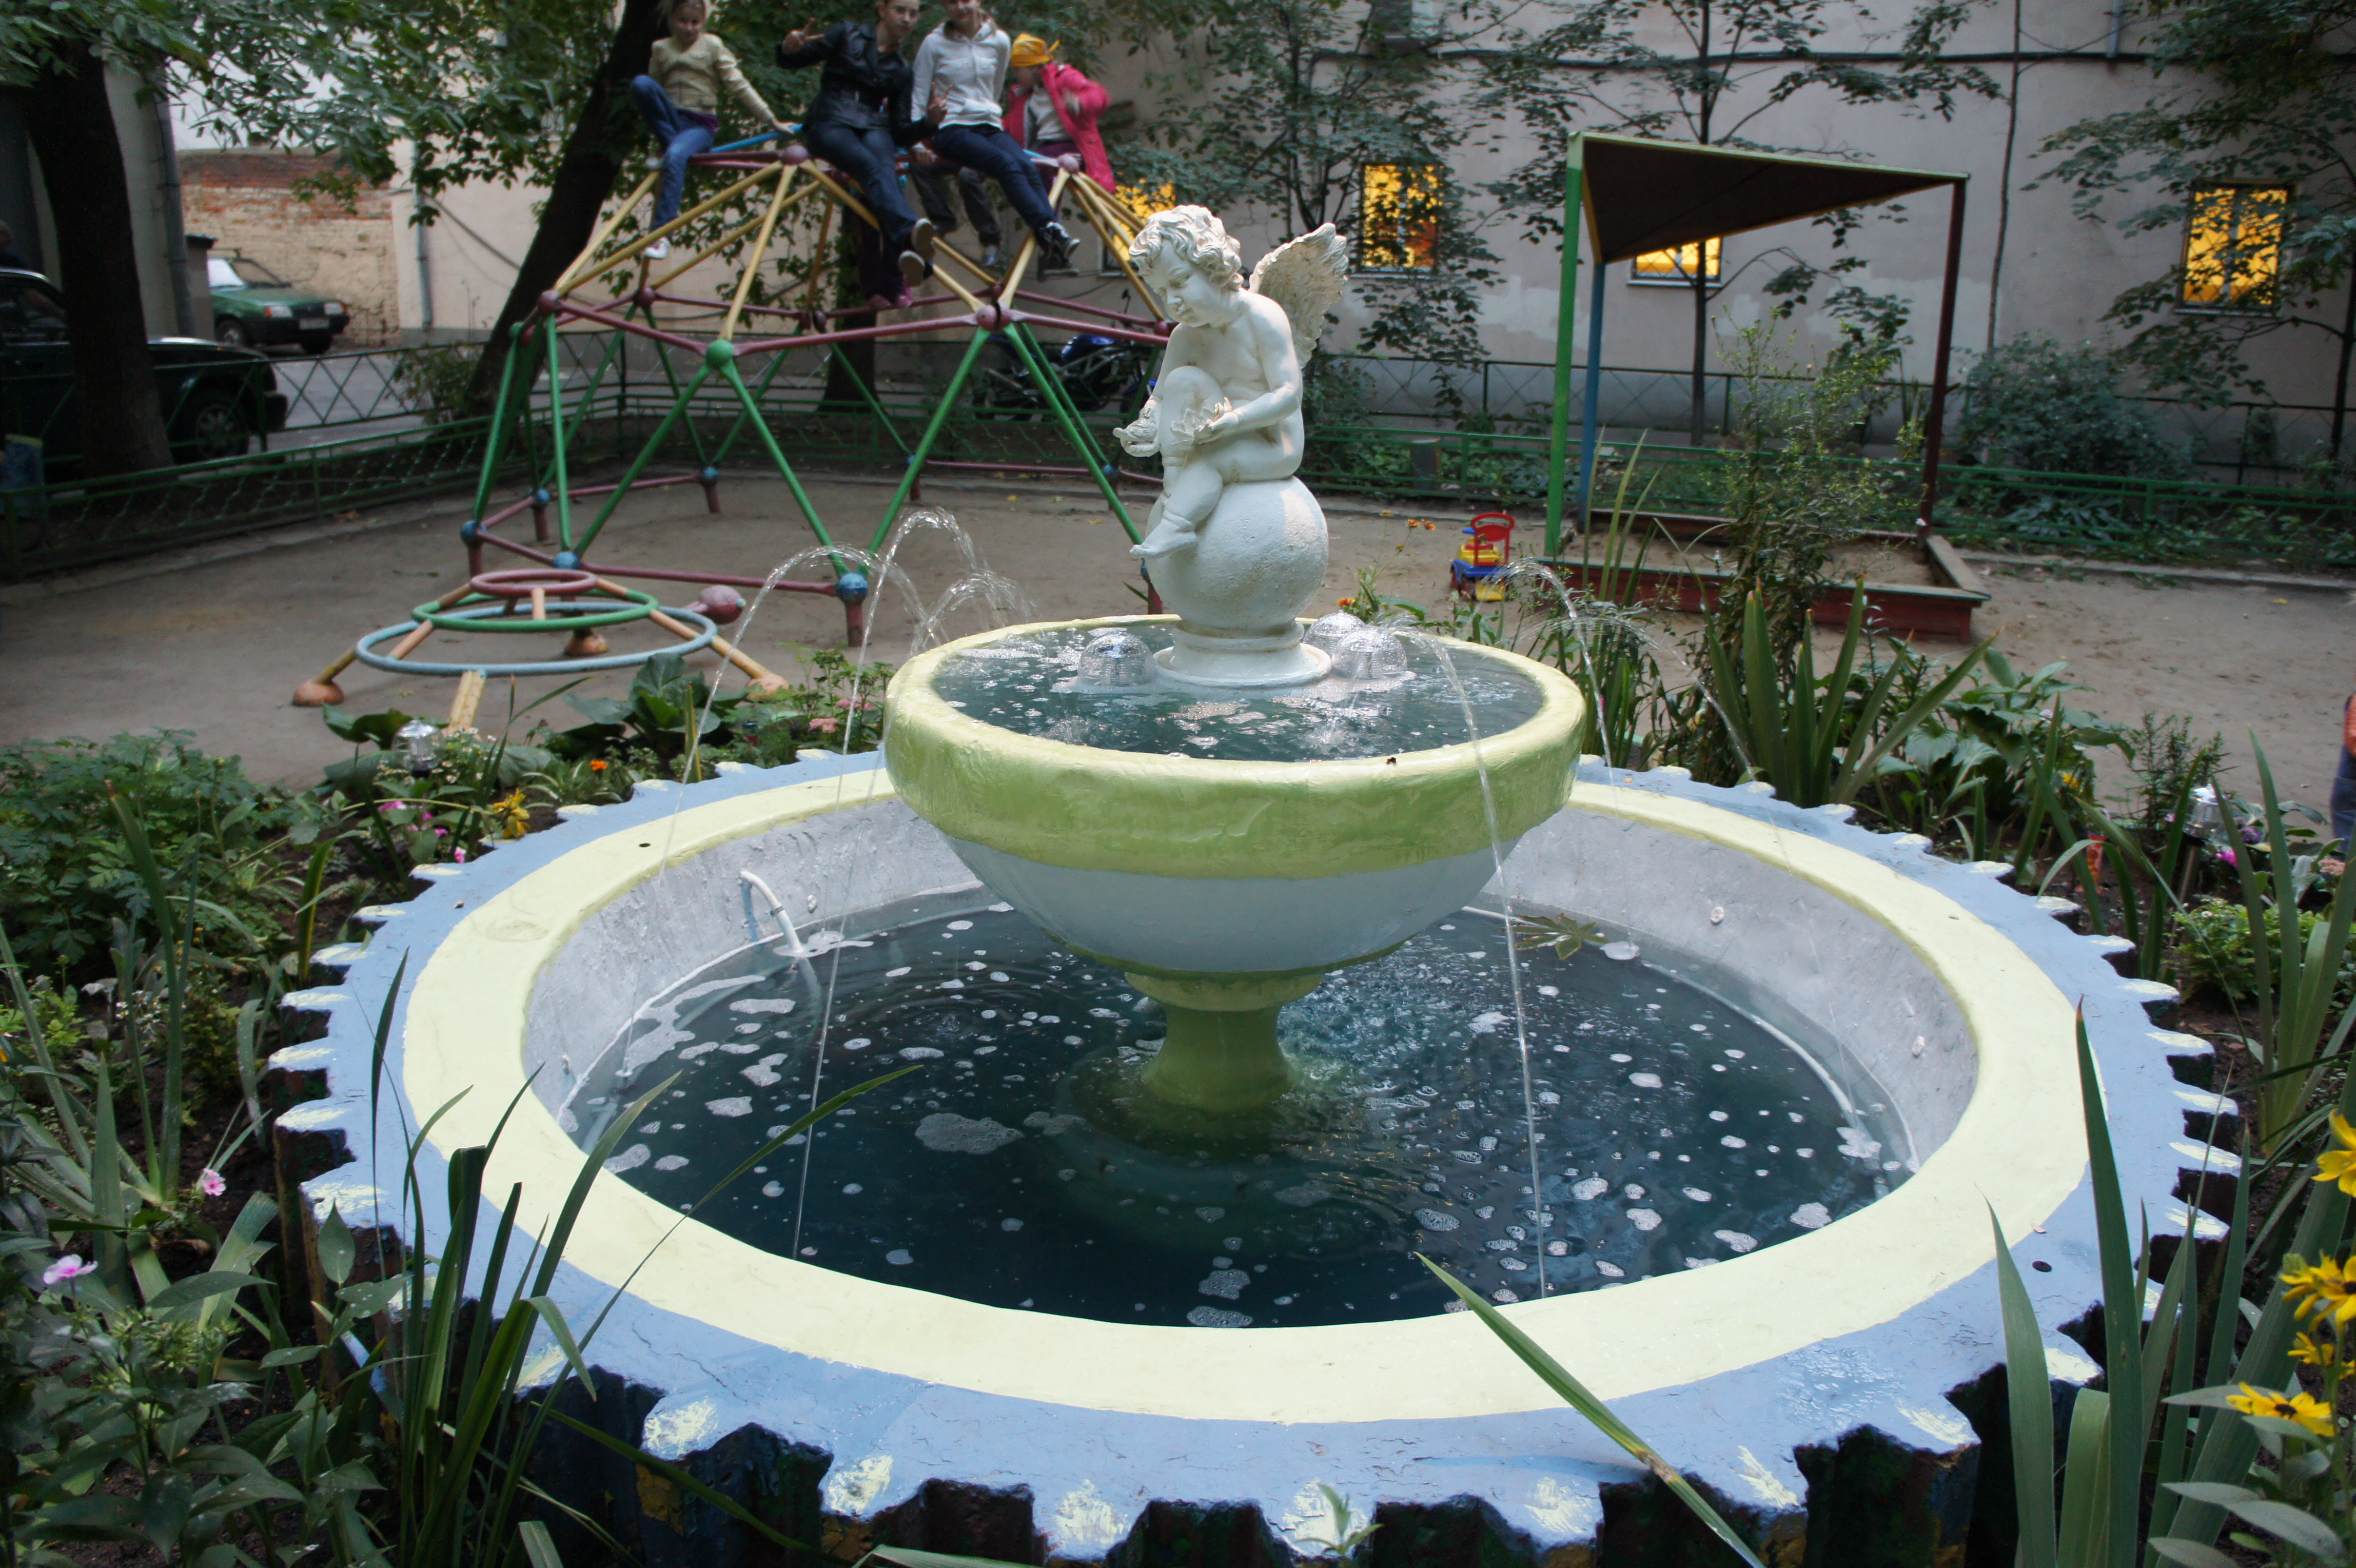
\includegraphics[width=100mm]{inc/85/2}
    \footnotesize{\textit{Сестры Клейн. Соня, Нина, Анжелика (Лика), Наташа (Туся). Конец 40-х.}}
\end{minipage}
\end{figure}
